\chapter{Filtering methods}
\label{sec:filter}

In this chapter, I present various filtering methods for approximate string matching.
I consider two classes of filtering methods: those based on \emph{seeds} and those based on \emph{$q$-grams}.
Filters of the former class partition the pattern into \emph{non-overlapping} factors called seeds, while filters of the latter class consider all \emph{overlapping} substrings of the pattern having length $q$, the so-called $q$-grams.
Both classes include various combinatorial filtering methods of increasing specificity and complexity; all methods provide filtration schemes with guarantees on filtration sensitivity.

I present two seed filtering methods:
%\begin{inparaenum}[(i)]
\emph{exact seeds} \citep{Baeza1992} and
\emph{approximate seeds} \citep{Myers1994,Navarro2000}.
%\emph{suffix filters} \citep{Kaerkkaeinen2007}.
%\end{inparaenum}
Exact seeds partition the pattern in $k+1$ non-overlapping seeds to be searched exactly in the text.
Approximate seeds increase filtration specificity by factorizing the pattern in less than $k+1$ non-overlapping seeds to be searched within a distance threshold smaller than $k$.
%Suffix filters further generalize exact and approximate seeds and yield stronger index based filtration.

I present the following $q$-gram filtering methods:
%\begin{inparaenum}[(i)]
\emph{contiguous $q$-grams} \citep{Jokinen1991},
\emph{gapped $q$-grams} \citep{Burkhardt2001} and
\emph{multiple gapped $q$-grams} (also called \emph{$q$-gram families}) \citep{Kucherov2005}.
%\end{inparaenum}
Contiguous $q$-grams rely on counting arguments to filter out text regions containing less than a given threshold of $q$-gram occurrences.
Gapped $q$-grams introduce \emph{don't care positions} to lower the correlation between occurrences of consecutive $q$-grams.
Multiple gapped $q$-grams adopt multiple patterns of don't care positions to further increase filtration specificity.

It will become clear through this chapter that seed filters are more practical, flexible, straightforward to design and implement than $q$-gram filters.
All seed filters provide full-sensitive filtration schemes for the $k$-differences problem, while (multiple) gapped $q$-grams only for $k$-mismatches.
The design of highly specific yet full-sensitive filtration schemes for $q$-gram filters is combinatorially hard, while it is quite straightforward for seed filters.
Also implementation-wise, $q$-gram filters are more involved than seeds filter.
In fact, seed filters lend themselves well to both online and offline variants of the problem, while $q$-gram filters are better suited for the online variant.
Finally, the experimental evaluation shows that seed filters outperform $q$-gram filters for most practical inputs.
For these reasons, I design the applications of chapters \ref{sec:masai} and \ref{sec:yara} around seed filtering methods.

%Problems of exact and approximate seeds filters are that: it is not evident which factorization yields optimal filtration, and they yield duplicate occurrences whenever errors are not distributed in the worst-case combination.
%The drawback is that the effort to implement them is slightly higher.

%In the following of this chapter I first present (multiple) gapped $q$-grams and problems associated with their design.
%Then I move to more practical approximate seeds, which I will adopt later in chapter~\ref{chap:map-eng}.
%Finally I discuss suffix filters and their practicality.

%Overall, through this chapter:
%\begin{itemize}
%\item I present a framework for the design of (multiple) gapped $q$-grams consisting of efficient exact and approximate solutions;
%\item I provide generic parallel implementations of filters based on exact and approximate seeds;
%\item I evaluate these filtration schemes in practice.
%\end{itemize}

% -----------------------------------------------------------------------------

\section{Exact seeds}
\label{sec:filtering:exact}

Filtration with exact seeds is one of the na\"ivest filtering methods for approximate string matching.
I first explain the underlying combinatorial principle, then I discuss implementation details and lastly give some insights on the efficiency of this method.

\subsection{Principle}

I consider the case of two arbitrary strings $\XSeq,\YSeq$ within edit distance $k$.
The generalization to $k$-differences is straightforward.

%If I partition \wlogs $\YSeq$ into $k+1$ non-overlapping seeds, then at least one seed will occur as a factor of $\XSeq$.
\begin{lemma}[Exact seeds]
\label{lemma:exact-seeds}
Let $\XSeq,\YSeq$ be two strings \st $d_E(\XSeq,\YSeq) = k$.
%If $\YSeq=y^1 y^2 \dots y^{k+1}$ then $\XSeq=ay^ib$ for some $a, b$.
If $\YSeq$ is partitioned \wlogs into $k+1$ non-overlapping seeds, then at least one seed occurs as a factor of $\XSeq$ \citep{Baeza1992}.
\end{lemma}
%\begin{proof}
%I proceed by induction on $k$.
%For $k=0$, the string $\YSeq$ is partitioned into one factor, $\YSeq$ itself.
%The condition $d_E(\XSeq,\YSeq) = 0$ implies $\XSeq=y$, which is true for $a=\epsilon$ and $b=\epsilon$.
%I suppose the case $k=j-1$ to be true, thus since $d_E(\XSeq,\YSeq) = j-1$ and $\YSeq=y^1 y^2 \dots y^{j}$ then $\XSeq=ay^ib$ for some $a, b$.
%I consider the case $k=j$. The $j$-th error can be in
%\begin{inparaenum}[(i)]
%\item\label{lemma:exact-seeds:prefix} $\YSeq^1\dots y^{i-1}$,
%\item\label{lemma:exact-seeds:infix} $\YSeq^i$, or
%\item\label{lemma:exact-seeds:suffix} $\YSeq^{i+1}\dots y^{j}$.
%\end{inparaenum}
%In case~\ref{lemma:exact-seeds:prefix} or~\ref{lemma:exact-seeds:suffix}, $\XSeq=ay^ib$ clearly holds.
%In case~\ref{lemma:exact-seeds:infix}, if I partition $\YSeq^i$ in two factors $\YSeq^{i'}$ and $\YSeq^{i''}$, then either $\XSeq=ay^{i'}b'$ or $\XSeq={a'}y^{i''}b$.
%\end{proof}
It is immediate to see that any edit distance error can cover at most one seed.
Therefore, at least one seed of $\YSeq$ will not be covered by any seed and hence occur as a factor of $\XSeq$.
Figure~\ref{fig:seeds-ext} shows an example.

This filtering method reduces the approximate search into multiple smaller exact searches.
It solves $k$-differences by partitioning the pattern into $k+1$ seeds, searching all seeds in the text, and verifying a text window around each occurrence of any seed in the text.
As lemma~\ref{lemma:exact-seeds} is valid for \emph{any substring} of the text within distance $k$ from the pattern, this method finds all approximate occurrences of the pattern in the text.

\begin{figure}[b]
\begin{center}
\caption[Filtration with exact seeds]{Filtration with 6 exact seeds solves $5$-differences. In the illustration, pattern $\Pattern$ occurs in text $\Text$ at edit distance 5. The seed in grey is not covered by any error and thus preserved.}
\label{fig:seeds-ext}
\begin{tikzpicture}[font=\normalsize]

\tikzstyle{n}=[inner sep=0pt, minimum size=10pt, align=center]
\tikzstyle{e}=[-latex, thin]
\tikzstyle{m}=[draw, shape=circle, clabel, pos=0.4, align=center, inner sep=0pt, minimum size=8pt, font=\tiny]
\tikzstyle{t}=[draw, shape=circle, clabel, pos=0.4, align=center, inner sep=0pt, minimum size=8pt, font=\tiny, fill=LightGray]
\tikzstyle{frame}=[draw, rectangle, thin, inner sep=0pt]
\tikzstyle{covered}=[draw, rectangle, thin, inner sep=0pt, fill=LightGray]
\tikzstyle{tape}=[fill=black]
\tikzstyle{strike}=[-, style=double, ultra thin, decorate, decoration=zigzag]
\tikzstyle{line}=[-, thin]
\tikzstyle{wave}=[-, thin, decorate, decoration={snake, segment length=2.5mm, amplitude=0.4mm}]


\newcommand{\transcript}[2]
{
    \foreach[count=\i] \r/\t/\g in {#2}
    {
    	\node[n] (read_\i) at (0.4*\i,0) {\r};
		\node[n] (genome_\i)  at (0.4*\i,-1) {\g};
		\ifthenelse{\equal{\t}{M}}
	    {
			\draw[e] (read_\i) -- (genome_\i) node[m] (transcript_\i) {\t};
		}
		{
			\draw[e] (read_\i) -- (genome_\i) node[t] (transcript_\i) {\t};
		}
    }
    
    \begin{pgfonlayer}{background} 
		\draw[tape] ([xshift=0.1cm, yshift=-0.01cm]transcript_1.north west) rectangle ([xshift=-0.1cm, yshift=0.01cm]transcript_#1.south east) ;
	\end{pgfonlayer}
}

\newcommand{\seed}[3]
{
	\ifthenelse{\equal{#3}{0}}
    {
%    	\draw[strike] (read_#1.west) -- (read_#2.east) ;

	    \begin{pgfonlayer}{background} 
    		\draw[covered] (read_#1.north west) rectangle (read_#2.south east) ;
		\end{pgfonlayer}
    }
           
	\node[frame] (read_rect) [transform shape, fit = (read_#1) (read_#2)] {};
}

\newcommand{\band}[1]
{
%	\node[frame] (genome_rect) [transform shape, fit = (genome_1) (genome_#1)] {};

	\draw[line] (genome_1.north west) -- (genome_#1.north east) ;
	\draw[line] (genome_1.south west) -- (genome_#1.south east) ;
	\draw[line] (genome_1.north west) -- (genome_1.south west) ;
	\draw[line] (genome_#1.north east) -- (genome_#1.south east) ;
}

\transcript{25}{G/M/G, C/M/C, T/M/T, N/R/A, T/M/T, G/M/G, G/D/$-$, G/M/G, C/M/C, A/M/A, T/M/T, T/M/T, A/R/G, T/M/T, G/M/G, G/M/G, C/M/C, $-$/I/C, C/M/C, A/M/A, T/M/T, T/M/T, T/M/T, T/R/A, T/M/T}
\band{25}

\node[left=0.25cm of read_1] {$x$} ;
\node[left=0.25cm of genome_1] {$y$} ;
\node[left=0.25cm of transcript_1] {$transcript$} ;

% (a) Exact seeds
% GCTN TGGG CATT ATGG C-CAT TTTT
% GCTA TG-G CATT GTGG CCCAT TTAT
%
\seed{1}{4}{0}
\seed{5}{8}{0}
\seed{9}{12}{1}
\seed{13}{16}{0}
\seed{17}{21}{0}
\seed{22}{25}{0}

% (b) Approximate seeds
% GCTNTGGG CATTATGG C-CATTTTT
% GCTATG-G CATTGTGG CCCATTTAT
%
%\seed{1}{8}{0}
%\seed{9}{16}{1}
%\seed{17}{25}{0}

\end{tikzpicture}
\end{center}
\end{figure}

%\subsection{Implementation}
%\subsubsection{Filtration step}
%Due to its simplicity, this filtering method lends itself to both online and offline implementations.
%In the online implementation, all seeds are preprocessed \eg in a  index.
%In the offline implementation, seeds are looked up in the text index.

%\subsubsection{Redundancy}
%
%Redundancy is a practical problem of seed filters.
%Whenever errors are not distributed according to a worst-case combination for lemma~\ref{lemma:exact-seeds}, more than one seed reports the same candidate location.
%For instance, if two errors fall in the same seed, then at least two seeds will occur exactly.
%
%In practice, redundancy can be avoided either before or after the verification step.
%In the first case, any diagonal in the implicit DP matrix identifies a distinct pattern occurrence to be verified only once.
%All candidate locations of a pattern have to be collected, then sorted by diagonal position and checked.
%Alternatively, if the verification algorithm is fast or the number of redundant candidate locations is low, it is more appealing to verify candidate locations directly.
%Any two pattern occurrences beginning or ending at the same location in the text are redundant.
%To avoid reporting duplicate occurrences, all pattern occurrences have to be collected, sorted and checked.
%
%How many redundant error configurations are produced by filtration with exact seeds?
%Here I consider the fraction of redundant error combinations, not the fraction of redundant candidate locations reported by the filter.
%For simplicity, I consider only combinations of exactly $k$ errors.
%Filtration has to cover all possible ways of distributing $k$ errors among $k+1$ seeds, that is $\binom{2k}{k}$ error combinations.
%However, a fixed seed covers all combinations where the seed itself contains no errors and all $k$ errors are distributed among the remaining $k$ seeds, \ie $\binom{2k-1}{k}$ error combinations.
%Thus the fraction of error combinations covered by filtration with exact seeds over the minimal ones is
%\begin{equation}
%\frac{(k+1)\binom{2k-1}{k}}{\binom{2k}{k}} = \frac{k+1}{2}.
%\end{equation}
%For instance, when $k=5$, filtration with exact seeds covers 3 times more combinations than required.

\subsection{Efficiency}
\label{sec:filtering:exact:efficiency}

The efficiency of this method strongly depends on the number of verifications.
% filtration time is always $\Oh(m)$.
It is straightforward to derive the expected number of verifications under the assumption of the text being generated according to the uniform Bernoulli model.
I introduce the random variable $C$, counting the number of occurrences of a word in a text.
The emission probability of any symbol in $\Sigma$ is $p = 1/\sigma$ and under \iid assumptions the emission (and occurrence) probability of any word of length $q$ is simply
\begin{eqnarray}
\Pr[C > 0] = \frac{1}{\sigma^q}
\end{eqnarray}
thus the expected number of occurrences of a seed of length $q$ in a text of length $n$ is
\begin{eqnarray}
E[C] = \sum_{i=0}^{n-q}{\Pr[C > 0]} = \frac{n - q + 1}{\sigma^q} \leq \frac{n}{\sigma^q}.
\end{eqnarray}

Lemma~\ref{lemma:exact-seeds} requires to partition the pattern into $k+1$ seeds but leaves the freedom to choose their length.
This leads to the problem of finding an optimal pattern partitioning that minimizes the expected number of verifications.
I fix\footnote{For simplicity I ignore that some seed could have length $\left \lceil \frac{m}{k+1} \right \rceil$.} the length of all seeds to be
\begin{eqnarray}
\label{eq:seed-len}
q=\left \lfloor \frac{m}{k+1} \right \rfloor
\end{eqnarray}
to minimize the expected number of occurrences of any seed.
Under these conditions, the expected number of verifications produced by filtration with exact seeds is
\begin{eqnarray}
E[V] = E[C] \cdot (k + 1) < \frac{n (k + 1)}{\sigma^q}.
\end{eqnarray}
Nonetheless, inputs of practical interest like genomes and natural texts do not fit well the uniform Bernoulli model.
On those texts, uniform seed length often leads to suboptimal filtration.

%\subsubsection{Expected sublinearity}
%I now turn to the effect of the error rate on the runtime of the resulting $k$-differences algorithm.
%For which error rate the resulting algorithm is expected to have \emph{sublinear} runtime?
%\citeauthor{Gusfield1997} gives a rough estimate to this question.
%If the classic $\Oh(m^2)$ DP algorithm of section~\ref{sub:introonline} is adopted to verify candidate locations, the expected runtime must be
%\begin{eqnarray}
%E[V] \cdot m^2 < cn
%\end{eqnarray}
%for some constant $c$.
%Substituting $E[V]$ and solving for $q$ yields
%\begin{eqnarray}
%q > \log_{\sigma}{\frac{m^3}{c}}
%\end{eqnarray}
%and since $q$ in equation~\ref{eq:seed-len} is a function of $\Plen$ and $k$, it follows that
%\begin{eqnarray}
%\epsilon = \frac{k}{m} < \frac{m}{\log_{\sigma}{m}}
%\end{eqnarray}
%is the error rate for which this $k$-differences algorithm has expected sublinear runtime.

% -----------------------------------------------------------------------------

\section{Approximate seeds}
\label{sec:seeds-apx}

The simple analysis of section~\ref{sec:filtering:exact:efficiency} shows that filtration specificity is strongly correlated to the seed length.
Therefore, the crux of designing a stronger filter lies into increasing the seed length while respecting full-sensitivity constraints.
\cite{Myers1994}, subsequently followed by \cite{Navarro2000}, proposed \emph{approximate seeds} as a practical and effective generalization of exact seeds that yield stronger filters for $k$-differences.
The key idea of filtration with approximate seeds is to reduce the approximate search into smaller approximate searches, as opposed to filtration with exact seeds that reduces the approximate search into smaller exact searches.

\subsection{Principle}

Again, I start by considering two arbitrary strings $\XSeq,\YSeq$ within edit distance $k$.
The result then holds for any substring of the text within distance $k$ from the pattern.
\begin{lemma}[Approximate seeds]
\label{lemma:apx-seeds}
Let $\XSeq,\YSeq$ be two strings \st $d_E(\XSeq,\YSeq) = k$.
If $\YSeq$ is partitioned \wlogs into $s$ non-overlapping seeds \st $1 \leq s \leq k+1$, then at least one seed occurs as a factor of $\XSeq$ within distance $\lfloor k/s \rfloor$ \citep{Myers1994,Navarro2000}.
\end{lemma}
To prove full-sensitivity it suffices to see that, if none of the seeds occurs within its assigned distance, the total distance must be greater than $s \cdot \lfloor k/s \rfloor = k$.
Figure~\ref{fig:seeds-apx} illustrates.

\begin{figure}[t]
\begin{center}
\caption[Filtration with approximate seeds]{Filtration with approximate seeds. A filtration scheme with thresholds $\mathbf{t} = (1,1,1)$ solves $5$-difference. In the illustration, pattern $\Pattern$ occurs in text $\Text$ at edit distance 5. The seed in grey is covered only by one error and thus preserved.}
\label{fig:seeds-apx}
\begin{tikzpicture}[font=\normalsize\sffamily]

\transcript{25}{G/M/G, C/M/C, T/M/T, N/R/A, T/M/T, G/M/G, G/D/$-$, G/M/G, C/M/C, A/M/A, T/M/T, T/M/T, A/R/G, T/M/T, G/M/G, G/M/G, C/M/C, $-$/I/C, C/M/C, A/M/A, T/M/T, T/M/T, T/M/T, T/R/A, T/M/T}{1}
\band{25}
\seed{1}{25}{1}

\node[left=0.25cm of read_1] {$p$} ;
\node[left=0.25cm of genome_1] {$t$} ;

\qgrama{1}{$\#$, $\#$, $\#$, $\#$, $\#$, $\#$, $\#$, $\#$}{1}{8}
\qgrama{9}{$\#$, $\#$, $\#$, $\#$, $\#$, $\#$, $\#$, $\#$}{1}{8}
\qgramai{17}{$\#$, $ $, $\#$, $\#$, $\#$, $\#$, $\#$, $\#$, $\#$}{1}{8}

\draw[strike] (qgram_1_4.north) -- (qgram_1_4.south) ;
\draw[strike] (qgram_1_7.north) -- (qgram_1_7.south) ;
\draw[strike] (qgram_9_5.center)  -- (qgram_9_5.south) ;
\draw[strike] (qgram_17_8.north) -- (qgram_17_8.south) ;

\end{tikzpicture}
\end{center}
\end{figure}

%\begin{lemma}
%\label{lemma:apx-seeds-var}
%Let $\XSeq,\YSeq$ be two strings \st $d_E(\XSeq,\YSeq) = k$.
%Partition $\YSeq$ into $s$ non-overlapping seeds $\YSeq^1, y^2, \dots, y^s$.
%Assign an arbitrary distance threshold $k_i$ to each seed $\YSeq^i$, satisfying the following constraint:
%\begin{equation}
%s + \sum_{i=1}^{s}{k_i} > k.
%\end{equation}
%Then at least one seed occurs as a factor of $\XSeq$ within distance $k_i$.
%\end{lemma}

\subsection{Filtration schemes}

Approximate seeds provide filtration schemes of variable specificity.
The fastest but weakest filtration scheme is given by $s=k+1$, while the most specific filtration is obtained for $s=1$ \ie perfect filtration scheme without any verification step.
Alternatively, filtration specificity is controlled by acting on the minimum seed length $q$.
Fixing $q$ yields $s = \lfloor m/q \rfloor$, or vice versa, fixing the number of seeds $s$ gives $q =\lfloor m/s \rfloor$.
Filtration specificity is expected to increase with seed length.

Lemma \ref{lemma:apx-seeds} assigns the same distance threshold to all seeds, yet this is not obligatory.
Hence, I give a more general definition of \emph{filtration scheme} for approximate seeds.
\begin{definition}[Filtration scheme]
A seeds filtration scheme is an integer vector $\mathbf{t} = (t_{\At{1}}, \dots, t_{\AtEnd{s}})$, where integer $\Threshold_i \in \N_0$ represents the threshold assigned to the $i$-th seed.
\end{definition}

\begin{lemma}
\label{lemma:apx-scheme}
Any filtration scheme $\mathbf{t} = (t_{\At{1}}, \dots, t_{\AtEnd{s}})$ \st
\begin{eqnarray}
s + \sum_{i=\At{1}}^{\AtEnd{s}} t_i > k
\end{eqnarray}
is full-sensitive for $k$-differences (and $k$-mismatches).
\end{lemma}
%I say that a \emph{full-sensitive} filtration scheme \emph{solves} a $k$-differences instance.

\begin{example}
\label{ex:seeds-apx-scheme}
The filtration schemes $(0,0,0,0,0)$, $(1,1,0)$, $(2,1)$, $(4)$ are full-sensitive for $4$-differences.
%or any their permutation
For instance, given a pattern of length $\Plen=100$, according to equation~\ref{eq:seed-len}, $q$ is respectively $20, 33, 50, 100$.
\end{example}

How to choose a \emph{good} filtration scheme in practice?
Both \cite{Myers1994} and \cite{Navarro2000} carried out involved analysis to estimate the optimal parameterization. \citeauthor{Navarro2000} find out that a number of seeds $s=\Theta(m/\log_{\sigma}{n})$ yields an overall time complexity sublinear for an error rate $\epsilon < 1 - e/\sqrt{\sigma}$.
\citeauthor{Myers1994} reports an analogous sublinear time when $q=\Theta(\log_{\sigma}{n})$ is the seed length.
Yet, these results do not necessarily translate into optimal filtration schemes in practice.
The parameterization depends on the full-text index, the verification algorithm, the statistical properties of the text.
Missing the optimal number of seeds by one often results in a runtime penalty of an order of magnitude.

Having established the number of seeds, or their length, thresholds have to be assigned.
Lemma \ref{lemma:apx-scheme} allows to assign arbitrary distance thresholds.
In practice, it is convenient to distribute distance thresholds evenly, as seeds with the highest threshold dominate the overall filtration time.
The most strict threshold assignment is to give distance $\lfloor k/s \rfloor$ to $(k \bmod{s}) + 1$ seeds and distance $\lfloor k/s \rfloor - 1$ to the remaining seeds \citep{Siragusa2013}.

%\subsection{Implementation}
%Online/Offline. Backtracking.

%\subsection{Counting}
%Maybe introduce the $k+s$ seeds counting principle?

% -----------------------------------------------------------------------------

%\section{Suffix filters}

% -----------------------------------------------------------------------------

\section{Contiguous $q$-grams}
\label{sec:filtering:qgrams-ext}

$q$-Gram filters rely on counting arguments to filter out text regions containing less than a given threshold of $q$-gram occurrences.
The first $q$-gram counting filter for approximate string matching has been proposed in \citep{Jokinen1991}.
Filters for more general alignment problems have been proposed and implemented in \emph{QUASAR} \citep{Burkhardt1999}, \emph{SWIFT} \citep{Rasmussen2006} and \emph{STELLAR} \citep{Kehr2011}.

\subsection{Principle}

The counting argument of contiguous $q$-gram filters is based on \emph{$q$-gram similarity}: the number of substrings of length $q$ common to two given strings.
The following lemma relates $q$-gram similarity to edit distance, by giving a \emph{lower bound} on the $q$-gram similarity of any two strings $\XSeq,\YSeq$ within edit distance $k$.
As for seed filters, this result then easily translates to $k$-differences.

\begin{lemma}[The $q$-gram lemma]
\label{lemma:qgrams}
Let $\XSeq,\YSeq$ be two strings \st $d_E(\XSeq,\YSeq) = k$ and assume \wlogs $|\XSeq| \leq |\YSeq|$ and $|\XSeq| = \Plen$. Then $\XSeq$ and $\YSeq$ have $q$-gram similarity $\tau_q(\Plen,k) \geq \Plen - q + 1 - kq$ \citep{Jokinen1991}.
\end{lemma}
The first part of the threshold function $\tau_q$ counts the number of $q$-grams of $\XSeq$ (\ie $\Plen - q + 1$), while the second part counts how many $q$-grams can be covered by $k$ errors (\ie at most $q$ per error, hence $kq$ in total).
The position of errors in the transcript solely determines which $q$-gram occurrences are affected or preserved.
The $q$-gram lemma considers one \emph{worst case} positioning of the errors that \emph{minimizes} the threshold.
Figure~\ref{fig:qgrams-ext} exemplifies.

\begin{figure}[h]
\begin{center}
\caption[Filtration with contiguous $q$-grams]{Filtration with contiguous $q$-grams. A filtration scheme $(q,\Threshold) = (4,2)$ solves the instance $(25,5)$. In the illustration, pattern $\Pattern$ of length 25 occurs in text $\Text$ at edit distance 5. In this worst-case positioning of the errors, the two grey $q$-grams are preserved.}
\label{fig:qgrams-ext}
\begin{tikzpicture}[font=\normalsize\sffamily]

\transcript{25}{G/M/G, C/M/C, T/M/T, N/R/A, T/M/T, G/M/G, G/M/G, G/D/$-$, C/M/C, A/M/A, T/M/T, A/R/G, T/M/T, T/M/T, G/M/G, A/R/G, G/M/C, C/M/C, C/M/C, G/R/A, T/M/T, T/M/T, T/M/T, A/M/A, T/M/T}{4}
\band{25}
\seed{1}{25}{1}

\node[left=0.25cm of read_1] {$\Pattern$} ;
\node[left=0.25cm of genome_1] {$\Text$} ;

% Unaffected q-grams ###-#
\foreach \x in {21,22}
{
	\pgfmathtruncatemacro{\y}{1+Mod(\x-1,4)}
	\qgram{\x}{$\#$, $\#$, $\#$, $\#$}{\y}{1}
}

% Covered q-grams ###-#
\foreach \x in {1,...,20}
{
	\pgfmathtruncatemacro{\y}{1+Mod(\x-1,4)}
	\qgram{\x}{$\#$, $\#$, $\#$, $\#$}{\y}{0}
}

% Strikes over covered q-grams
\foreach \x in {1,...,20}
{
	\pgfmathtruncatemacro{\y}{4-Mod(\x-1,4)}
	\draw[strike] (qgram_\x_\y.north) -- (qgram_\x_\y.south) ;
}

\end{tikzpicture}
\end{center}
\end{figure}

\subsection{Filtration schemes}
\label{sec:filtering:qgrams-ext:schemes}

I denote by a pair $(q,\Threshold)$ the filtration scheme counting $q$-grams with threshold $\Threshold$.
According to lemma \ref{lemma:qgrams}, if $\Threshold = \tau_q(\Plen,k) \geq 1$, then $(q,\Threshold)$ is full-sensitive for any $k$-differences instance where $|\Pattern|=\Plen$.
In this case, I say that $(q,\Threshold)$ \emph{solves} instance $(\Plen,k)$.

The following question arises: which is the longest $q$-gram solving instance $(\Plen,k)$?
In order to satisfy lemma~\ref{lemma:qgrams}, the $q$-gram threshold must be greater than zero, \ie it must hold $\tau_q(\Plen,k) \geq 1$.
Thus, by substituting $\tau_q(\Plen,k)$, it follows that the $q$-gram length must be $q \leq \left \lfloor \frac{m}{k+1} \right \rfloor$, analogously to seed filters (see equation~\ref{eq:seed-len}).

However, the longest $q$-gram does not yield always the most specific filtration scheme.
For instance, a threshold of 1 completely discards the counting argument of lemma~\ref{lemma:qgrams} and makes filtration very unspecific in practice.
Hence, on certain $(\Plen,k)$ instances, filtration schemes with non-optimal $q$-gram length yield more specific filtration.
Example \ref{ex:qgrams-ext-scheme} shows alternative filtration schemes solving a given $(\Plen,k)$ instance.

\begin{example}
\label{ex:qgrams-ext-scheme}
The following $(q,\Threshold)$ filtration schemes solve $(100,4)$-differences:
$(20,1)$, $(19,6)$, $(18,11)$.
%or any their permutation
\end{example}

%\subsection{Implementation}
\subsection{Bucketing}

Filtration with $q$-grams requires \emph{bucketing} the text in windows, in order to apply the counting argument of lemma \ref{lemma:qgrams}.
Buckets are obtained by subdividing the implicit DP matrix in parallelograms and projecting them on the text.
Figure \ref{fig:swift} illustrates this concept: any approximate occurrence of the pattern in the text spans at most $k$ diagonals and is thus enclosed inside a parallelogram of width $k+1$ \citep{Rasmussen2006}.
Hence the projection of any text bucket has length $2k + 1$ and any occurrence has length between $\Plen - k$ and $\Plen + k$.
The implementations described in \citep{Rasmussen2006, Kehr2011, Weese2009} use more efficient bucketing strategies with larger, overlapping parallelograms.

\begin{figure}[h]
\begin{center}
\caption[Parallelogram buckets] {Parallelogram buckets. Picture from \citep{Weese2009}.}
\label{fig:swift}
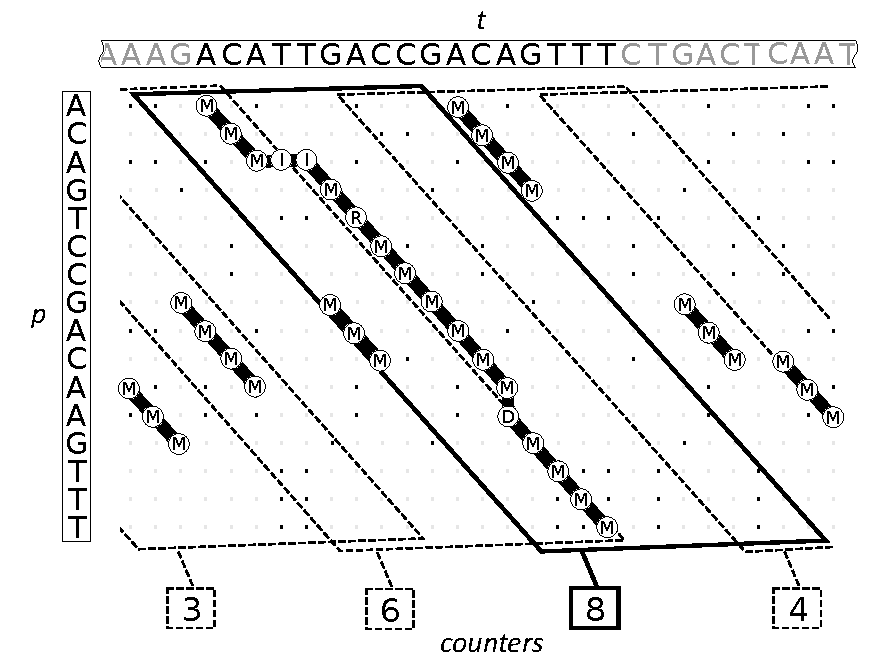
\includegraphics[scale=0.75]{figures/swift.pdf}
\end{center}
\end{figure}

This method lends itself to work in a multiple online fashion rather than offline.
The filtration stage scans the text and counts how many $q$-grams of each pattern fall into each parallelogram bucket.
As long as the filter scans the text, it remembers only the buckets that span the patterns' lengths.
The verification stage then verifies only those parallelograms exceeding threshold $\Threshold$.
Conversely, the program QUASAR \citep{Burkhardt1999} uses a $q$-gram index of the text to speed up the filtration phase.
Such implementation requires more memory, as it must bucket the whole text and keep the text index in memory.

% -----------------------------------------------------------------------------

\section{Gapped $q$-grams}
\label{sec:filtering:qgrams-gapped}

\cite{Califano1993} first introduced \emph{gapped $q$-grams} in sequence analysis.
Since then, a surprisingly high number of research papers have been published on this topic (see \citep{Brown2008} for a survey).
Almost all works focus on lossy filtration for homology search, rather than full-sensitive filtration for approximate string matching.
Here, I consider gapped $q$-grams only in the context of full-sensitive filtration for $k$-mismatches.
This case has been first considered by \cite{Burkhardt2001}.

\subsection{Principle}

Gapped $q$-grams introduce fixed \emph{don't care positions} where text and pattern characters are ignored.
A comparison between figures \ref{fig:qgrams-ext} and \ref{fig:qgrams-gapped} illustrates the advantage of such don't care positions.
While in figure \ref{fig:qgrams-ext} an error in a transcript affects (at most) a cluster of $q$ consecutive $q$-gram occurrences, in figure \ref{fig:qgrams-gapped} a mismatch does not affect those gapped $q$-gram occurrences that ignore its position.
This fact relaxes the full-sensitivity threshold and opens the door to more specific filtration schemes for $k$-mismatches.
%Note that insertions and deletions still affect don't care positions, hence $Q$-grams do not solve $k$-differences.
%Note how the occurrence of each contiguous $q$-gram is strongly correlated to the preceding and following ones.
%\emph{gapped $q$-grams} lower the correlation between the occurrences of consecutive $q$-grams.

The counting argument of gapped $q$-grams generalizes $q$-gram similarity (section~\ref{sec:filtering:qgrams-ext}) from substrings to \emph{subsequences}, \ie from contiguous to \emph{non-contiguous} sequences of symbols.
Filtration with gapped $q$-grams indeed counts the number of subsequences of length $q$ common to two strings.
An additional set $Q$ determines which symbols are taken in the subsequences.
The formal definition of gapped $q$-gram follows.

\begin{definition}[$Q$-gram]
A gapped $q$-gram (abbreviated as $Q$-gram) is a finite sequence $Q$ of natural numbers starting with the unit element, \ie $Q \subset \N_0$ and $\Ibase \in Q$.
The length $|Q|$ is called the \emph{weight} of $Q$ and denoted as $\Weight{Q}$.
The maximum element of $Q$ is named \emph{span} and indicated by $\Span{Q}$.
\end{definition}
%In literature, $Q$-grams are visualized as words over the alphabet $\{1,*\}$ or $\{\#,-\}$.
%I adopt the former notation and represent the $Q$-gram by the word $w \in \{1,*\}^{\Span{Q}}$ such that $w_j=1$ iff $j \in Q$.

Figure~\ref{fig:qgrams-gapped} shows an example of $Q$-gram.
As in lemma \ref{lemma:qgrams}, the threshold for $Q$-grams still depends on the worst-case positioning of the errors in the transcript, which in turn depends on parameters $(\Plen,k)$.
Thus, I still consider filtration schemes $(Q,\Threshold)$ solving a $(\Plen,k)$ instance.
However, contrary to contiguous $q$-grams, function $\tau_Q$ now gives only a lower bound to the full-sensitivity threshold.

\begin{figure}[t]
\begin{center}
\caption[Filtration with gapped $q$-grams]{Filtration with gapped $q$-grams. A filtration scheme $(Q,\Threshold) = (\{\At{1}, \At{3}, \At{4}, \At{5}\},3)$ solves instance $(25,5)$. In the illustration, pattern $\Pattern$ of length 25 occurs in text $\Text$ at edit distance 5. The three $q$-grams in grey are not covered by any mismatch.}
\label{fig:qgrams-gapped}
\begin{tikzpicture}[font=\normalsize\sffamily]

\transcript{25}{G/1/G, C/1/C, T/1/T, T/1/T, N/0/A, G/1/G, T/1/T, G/1/G, C/1/C, G/0/A, T/1/T, A/1/A, T/1/T, T/1/T, A/0/G, A/1/A, G/1/C, C/1/C, C/1/C, G/0/A, T/1/T, T/1/T, A/0/T, A/1/A, T/1/T}{5}
\band{25}
\seed{1}{25}{1}

\node[left=0.25cm of read_1] {$\Pattern$} ;
\node[left=0.25cm of genome_1] {$\Text$} ;

% Unaffected q-grams ###-#
\foreach \x in {4,9,14}
{
	\pgfmathtruncatemacro{\y}{1+Mod(\x-1,5)}
	\qgramg{\x}{$\#$, $ $, $\#$, $\#$, $\#$}{\y}{1}
}

% Covered q-grams ###-#
\foreach \x in {1,2,3,5,6,7,8,10,11,12,13,15,16,17,18,19,20,21}
{
	\pgfmathtruncatemacro{\y}{1+Mod(\x-1,5)}
	\qgramg{\x}{$\#$, $ $, $\#$, $\#$, $\#$}{\y}{0}
}

% Strikes over covered q-grams
\foreach \x in {1,2,3,5,6,7,8,10,11,12,13,15,16,17,18,20}
{
	\pgfmathtruncatemacro{\y}{5-Mod(\x-1,5)}
	\draw[strike] (qgram_\x_\y.north) -- (qgram_\x_\y.south) ;
}
\draw[strike] (qgram_21_3.north) -- (qgram_21_3.south) ;
\draw[strike] (qgram_20_4.north) -- (qgram_20_4.south) ;
\draw[strike] (qgram_19_5.north) -- (qgram_19_5.south) ;

\end{tikzpicture}
\end{center}
\end{figure}


\subsection{Filtration schemes}
\label{sub:qgram:design}

Which is the most specific filtration scheme $(Q,\Threshold)$ solving a given instance $(\Plen,k)$?
This question turns out to be surprisingly hard to answer.
As discussed in section \ref{sec:filtering:qgrams-ext:schemes}, the most specific filtration schemes for contiguous $q$-grams are easily found.
The choice falls on a few values of $q$ that are close to the maximum and do not yield a threshold too close to $1$.
Conversely, such choice is non-trivial for $Q$-grams, as the search space of $Q$ is exponentially large in the span $\Span{Q}$ and a full-sensitivity threshold for arbitrary $Q$-grams is hard to compute.
In addition, it is not easy to determine which filtration scheme is the most specific one in a set of full-sensitive candidates.

%The design of $Q$-gram filtration schemes raises hard combinatorial problems.
Given a $Q$-gram, I consider the following problems:
\begin{table}[h]
\begin{tabular}{rl}
\textsc{Full Sensitivity} & Does filtration scheme $(Q,1)$ solve instance $(\Plen,k)$?\\
\textsc{Optimal Threshold} & Which is the optimal threshold $\Threshold^*$ \st $(Q,\Threshold^*)$ solves $(\Plen,k)$?\\
\textsc{Specificity} & Which is the expected specificity of scheme $(Q,\Threshold)$?\\
\end{tabular}
\end{table}
%\label{enum:qgram-distance} Which is the minimum distance $k^*$ for which $(\Plen,k^*)$ is not solved by $(Q,\Threshold)$?

\cite{Nicolas2005} considered the decision problem \textsc{Full Sensitivity} associated to \textsc{Optimal Threshold}.
\textsc{Full Sensitivity} is easy for contiguous $q$-grams, \ie the answer is no iff $\tau_q(\Plen,k) = 0$.
\citeauthor{Nicolas2005} show, by performing an indirect reduction from \textsc{Exact Cover by 3-Sets}, that \textsc{Full Sensitivity} is \emph{strongly} NP-complete for arbitrary $Q$-grams.
Strong NP-completeness implies that no \emph{fully polynomial-time approximation scheme} (FPTAS) nor any \emph{pseudo-polynomial} algorithm for \textsc{Full Sensitivity} exist, under the assumption that $P \neq NP$.

\cite{Burkhardt2001} first considered the optimization problem \textsc{Optimal Threshold}.
They give a DP algorithm solving \textsc{Optimal Threshold} in time $\Oh(m \cdot k \cdot 2^{\Span{Q}})$ for any $Q$-gram.
Subsequently, they use their DP algorithm to explore the search space of full-sensitive $Q$-grams for some specific instances of $(\Plen,k)$.
They reduce the search space using a \emph{branch-and-bound} algorithm based on the observation that:
\begin{eqnarray}
Q_1 \subseteq Q_2 \iff \tau_{Q_1}(\Plen,k) \geq \tau_{Q_2}(\Plen,k).
\end{eqnarray}
Finally, \citeauthor{Burkhardt2001} guess the most specific filtration scheme $(Q,\Threshold)$ by computing, again via branch-and-bound, the minimum number of characters covered by $\Threshold$ distinct $Q$-gram occurrences (\textsc{Minimum Coverage} criterion).

I propose alternative algorithms for the design of $Q$-gram filtration schemes.
I give an \emph{integer linear program} (ILP) that solves exactly \textsc{Optimal Threshold} and is orders of magnitude quicker than the DP algorithm from \citep{Burkhardt2001} (see table~\ref{tab:threshold}).
Afterwards, I give a simple polynomial time \emph{approximation algorithm} for \textsc{Optimal Threshold} usable as an additional search space filter to quickly discard lossy $Q$-grams and eventually providing good ILP starting points.
Finally, I propose a randomized algorithm to estimate in polynomial time the specificity of a filtration scheme, instead of using the \textsc{Minimum Coverage} criterion.

Having said that, I have no practical interest into designing $Q$-gram filtration schemes.
On the one hand, almost all HTS applications require methods that solve $k$-differences in order to detect indels.
On the other hand, the experimental evaluation of section \ref{sec:filtering:evaluation} shows that $Q$-gram filters are not better than approximate seeds filters.
Therefore, I do not need these algorithms in the applications presented in chapters~\ref{sec:masai} and \ref{sec:yara}.

\subsection{Full sensitivity}
\label{sub:qgram-non-detection}

I start by modeling the decision problem \textsc{Full Sensitivity} before turning to the optimization problem \textsc{Optimal Threshold}.
I consider any Hamming distance transcript over $\{ \text{\ttfamily R}, \text{\ttfamily M} \}$ as an $\Plen$-dimensional vector $\mathbf{x} = (x_{\At{1}}, \dots x_{\AtEnd{\Plen}})$ over $\Bo = \{ 0, 1 \}$.
Accordingly, I denote by $|\mathbf{x}|_0=\Plen - \sum \mathbf{x}$ the Hamming distance of the transcript, and by $\Bo^{\Plen}_k \subset \Bo^{\Plen}$ the set containing all transcripts $\mathbf{x}$ \st $|\mathbf{x}|_0 = k$.
I now define the event of detection of a transcript by a filtration scheme $(Q,\Threshold)$.

\begin{definition}
\label{def:qgram-occ}
A $Q$-gram \emph{occurs} at position $i$ in a transcript $\mathbf{x}$ iff $\forall j \in Q$ $x_{i+j}=1$.
\end{definition}

\begin{definition}
\label{def:qgram-detection}
A filtration scheme $(Q,\Threshold)$ \emph{detects} $\mathbf{x}$ iff the $Q$-gram occurs at least $\Threshold$ times in $\mathbf{x}$.
\end{definition}

I introduce a \emph{boolean function} to characterize the set of transcripts detected by a filtration scheme of the form $(Q,1)$.
Let $T_{Q}^{m}: \Bo^{\Plen} \rightarrow \Bo$ denote the boolean function such that $T_{Q}^{m}(\mathbf{x})$ is true iff the $Q$-gram occurs in a transcript $\mathbf{x}$ of length $\Plen$.
I define such boolean function as the disjunction
\begin{equation}
\label{eq:qgram-bool}
T_{Q}^{m}(\mathbf{x}) = \bigvee_{i=\At{1}}^{\Plen-\Span{Q}} \bigwedge_{j \in Q} x_{i+j}
\end{equation}
where each \emph{clause} of $T_{Q}^{m}$ represents a single possible occurrence of $Q$ in $\mathbf{x}$.
According to definition \ref{def:qgram-detection}, filtration scheme $(Q,\Threshold)$ detects $\mathbf{x}$ iff $\mathbf{x}$ satisfies at least $\Threshold$ clauses of $T_{Q}^{m}$.
The formal definition of \textsc{Full Sensitivity} follows.

%The utility of these functions is manyfold.
%In section \ref{sub:qgram-optimal-threshold}, I use them within an ILP that computes an exact solution to \textsc{Optimal Threshold} and thus answers \textsc{Full Sensitivity}.
%In section \ref{sub:qgram-specificity}, I reduce the estimation of filtration sensitivity to a counting problem on boolean functions.

\begin{problem}[\textsc{Full Sensitivity}]
\begin{tabular}{rl}
{\bf Instance}	&	A $Q$-gram, an $(\Plen,k)$ instance. \\
{\bf Question}	&	$\exists \, \mathbf{x} \in \Bo^{\Plen}_k$ \st $T_{Q}^{m}(\mathbf{x}) = 0$? \\
\end{tabular}
\end{problem}


\subsection{Optimal threshold}
\label{sub:qgram-optimal-threshold}

I now consider the \emph{pseudo-boolean function}, counterpart of function \ref{eq:qgram-bool}, that associates a filtration threshold to any transcript.
Let the function $\Threshold_{Q}^{m}: \Bo^{\Plen} \rightarrow \N_0$ be the boolean function $T_{Q}^{m}$ acting on $\N_0$.
Here, $\Threshold_{Q}^{m}(\mathbf{x})$ \emph{counts} how many times a $Q$-gram occurs in a transcript $\mathbf{x}$ of length $\Plen$.
I define such pseudo-boolean function as
\begin{equation}
\label{eq:qgram-pseudo}
t_{Q}^{m}(\mathbf{x}) = \sum_{i=\At{1}}^{\Plen-\Span{Q}} \prod_{j \in Q} x_{i+j}
\end{equation}
The formal definition of \textsc{Optimal Threshold} follows.

\begin{problem}[\textsc{Optimal Threshold}]
\begin{tabular}{rl}
{\bf Instance}	&	A $Q$-gram, an $(\Plen,k)$ instance.\\
{\bf Solution}	&	$\min \, t_{Q}^{m}(\mathbf{x})$ subject to $\mathbf{x} \in \Bo^{\Plen}_k$
\end{tabular}
\end{problem}

\subsubsection{Exact solution}

I propose the following ILP to solve \textsc{Optimal Threshold}.
%The complementary \textsc{optimal threshold} is \textsc{maximum coverage} \citep{Vazirani2001}.

\begin{equation}
\begin{array}{lll}
\min & \sum \mathbf{t}							\\
\text{subject to}								\\
& \mathbf{t} \in \Bo^{\Plen - \Span{Q} + 1}		\\
& \mathbf{x} \in \Bo^{\Plen}_k					\\
& t_i \geq x_{i+j} 						& \forall \, \At{1} \leq i \leq \Plen-\Span{Q} \quad \quad \forall \, j \in Q \\
\end{array}
\end{equation}

Vector $\mathbf{t}$ represents function $T_{Q}^{m}$ and its sum function $\Threshold_{Q}^{m}$; each $\Threshold_i$ indicates the truthfulness of the $i$-th clause of $T_{Q}^{m}$.
Vector $\mathbf{x}$ represents any Hamming transcript; each $x_j$ is subject to an integer linear constrain \st the Hamming distance of $\mathbf{x}$ is within $k$.
The set of inequalities of the form $\Threshold_i \geq x_{i+j}$ binds the satisfiability of each clause $\Threshold_i$ to its associated transcript values $x_j$.
The solution $\mathbf{t}^*$ to the above ILP provides the optimal threshold $\Threshold=\sum \mathbf{t}^*$ for a $Q$-gram on instance $(\Plen,k)$.

\subsubsection{Approximate solution}

Pseudo-boolean function $\Threshold_{Q}^{m}$ has two important properties: it is \emph{monotone non-decreasing} and \emph{supermodular}.
In particular, supermodularity is the discrete analog of concavity.
These properties allow to compute approximate solutions to constrained optimization problems in polynomial time.
A pseudo-boolean function $f : \mathbb{B}^{\Plen} \rightarrow \mathbb{Z}$ is monotone non-decreasing iff 
\begin{equation}
\label{eq:monotone-non-decreasing}
f(\mathbf{y}) \leq f(\mathbf{y} \vee \mathbf{z}) \quad \forall \, \mathbf{y}, \mathbf{z} \in \mathbb{B}^{\Plen}
\end{equation}
and it is \emph{supermodular} iff 
\begin{equation}
\label{eq:supermodularity}
f(\mathbf{y}) + f(\mathbf{z}) \leq f(\mathbf{y} \vee \mathbf{z}) + f(\mathbf{y} \wedge \mathbf{z}) \quad \forall \, \mathbf{y}, \mathbf{z} \in \mathbb{B}^{\Plen}.
\end{equation}
%or, equivalently, if all its second order derivatives are non-negative, \ie
%\begin{equation}
%\label{eq:supermodularity-partial}
%\frac{\partial^2 f}{\partial z_i \partial z_j}(\mathbf{z}) \geq 0 \quad \forall \, \mathbf{z} \in \mathbb{B}^{\Plen} \text{ and } \forall \, 1 \leq i \leq j \leq m
%\end{equation}
It is immediate to see that function $\Threshold_{Q}^{m}$ satisfies all the above inequalities, as it does not contain any term in negative form by definition (see equation \ref{eq:qgram-pseudo}).
\textsc{Optimal Threshold} thus involves the minimization of a monotone supermodular function subject to linear constraints.

There is a well-known \emph{gradient ascent} algorithm for the maximization of a monotone submodular function subject to linear constraints with an APX-ratio of $1 - 1/e$ \citep{Nemhauser1978}, \ie the ratio between the value of the greedy approximation and the value of the optimal solution is within $0.632$.
Algorithm~\ref{alg:qgram-threshold-apx} computes an approximate solution to \textsc{Optimal Threshold} using the same principle.
Nonetheless, its solution is not guaranteed to be within a constant ratio from the optimal one.
Indeed, algorithm~\ref{alg:qgram-threshold-apx} minimizes function $\Threshold_{Q}^{m}$ which is monotone non-decreasing supermodular and has its unconstrained minimum at $0$.

In practice, the threshold found by algorithm~\ref{alg:qgram-threshold-apx} turns out to be a tight upper bound for \textsc{Optimal Threshold} (see table~\ref{tab:threshold}).
Such threshold cannot be used in a filtration scheme guaranteed to be full-sensitive: if the threshold is non-optimal, the filtration scheme is lossy.
Instead, algorithm~\ref{alg:qgram-threshold-apx} might find its use in the design of $Q$-grams, as a search space filter to quickly discard lossy $Q$-grams.

%I define the negated function $\bar{t}_{Q}^{m}$, counting how many times a $Q$-gram does not occur in a transcript $\mathbf{x}$, as
%\begin{equation}
%\label{eq:qgram-pseudoneg}
%\bar{t}_{Q}^{m}(\mathbf{x}) = m - \Span{Q} + 1 - t_{Q}^{m}(\mathbf{x})
%\end{equation}
%Function $\bar{t}_{Q}^{m}$ is monotone non-increasing and submodular.
%I consider the complementary problem, being the maximization of a submodular function subject to linear constraints:
%{\bf Solution}	&	$\max \, \bar{t}_{Q}^{m}(\mathbf{x})$ \wrt $\mathbf{x} \in \bar{\Bo}^{\Plen}_k$

\begin{figure*}[b]
\begin{center}
\begin{minipage}[t]{.8\textwidth}
\begin{algorithm}[H]
\Algorithm{ApproximateThreshold}{$Q,\Plen,k$}
\begin{tabular}{ll}
\textbf{Input}  & $Q$ : $Q$-gram\\
				& $\Plen$ : integer denoting the pattern length\\
				& $k$ : integer bounding the number of mismatches\\
\textbf{Output} & integer indicating the optimal threshold\\
\end{tabular}
\begin{algorithmic}[1]
\State {$\mathbf{x} \gets \mathbf{1}^{\Plen}$}
\While {$k > 0$}
	\State {i \gets $ \argmax_{j=1}^{m} \frac{\partial t^{\Plen}_Q(\mathbf{x})}{\partial x_j}$}
%	\State {i \gets $ \argmax_{j=1}^{m} \frac{\partial \bar{t}^{\Plen}_Q(\mathbf{x})}{\partial x_j}$}
	\State {$x_i \gets 0$}
	\State {$k \gets k - 1$}
\EndWhile
\State \Return $\Threshold^{\Plen}_Q(\mathbf{x})$
%\State \Return $\Plen - \Span{Q} + 1 - \bar{t}^{\Plen}_Q(\mathbf{x})$
\end{algorithmic}
\label{alg:qgram-threshold-apx}
\end{algorithm}
\end{minipage}
\end{center}
\end{figure*}


\subsection{Specificity}
\label{sub:qgram-specificity}

Assuming the text to be generated according to the uniform Bernoulli model, the expected specificity of any filtration scheme is proportional to the number of transcripts detected.
Thus, among multiple full-sensitive filtration schemes, one clearly prefers the one that minimizes the number of transcripts detected.

\begin{problem}[\textsc{Specificity}]
\begin{tabular}{rl}
{\bf Instance}	&	A filtration scheme $(Q,\Threshold)$, an $(\Plen,k)$ instance.\\
{\bf Solution}	&	$| \{ \mathbf{x} \in \Bo^{m} : t_{Q}^{m}(\mathbf{x}) \geq t \} |$
\end{tabular}
\end{problem}

\subsubsection{Approximate solution}

I propose a \emph{fully polynomial-time randomized approximation scheme} (FPRAS) \citep{Vazirani2001} to estimate the number of transcripts detected by a filtration scheme of the type $(Q,1)$.
This number coincides with the number of true assignments to the boolean function $T_{Q}^{m}$, \ie $| \{ \mathbf{x} \in \Bo^{m} : T_{Q}^{m}(\mathbf{x}) \} |$.
Boolean function $T_{Q}^{m}$, as defined in equation \ref{eq:qgram-bool}, is in \emph{disjunctive normal form} (\emph{DNF}).
Counting the number of true assignments to an arbitrary boolean function in DNF is a classic \emph{\#P-complete} problem, that however allows approximability to any degree \citep{Vazirani2001}.

Algorithm~\ref{alg:qgram-specificity} follows the algorithm in \citep{Karp1989} to estimate the number of true assignments of an arbitrary boolean function in DNF.

\begin{figure*}[b]
\begin{center}
\begin{minipage}[t]{.8\textwidth}
\begin{algorithm}[H]
%\Algorithm{CountTranscripts}{$Q,\Threshold,\Plen,\epsilon$}
\Algorithm{CountTranscripts}{$Q,\Plen,\epsilon$}
\begin{tabular}{ll}
\textbf{Input}  & $Q$ : $Q$-gram\\
%				& $\Threshold$ : integer denoting the threshold\\
				& $\Plen$ : integer denoting the pattern length\\
				& $\epsilon$ : real $\in [0,1]$ denoting the approximation factor\\
\textbf{Output} & integer indicating the number of transcripts detected\\
\end{tabular}
\begin{algorithmic}[1]
\State $C \gets \Plen+\Span{Q}+1$
\State $M \gets C \cdot 2^{\Plen-\Weight{Q}}$
\State $N \gets 4 \cdot C^2 / \epsilon^2$
\State $T \gets 0$
\Repeat
	\State {$i \gets$ \Call{random}{$\OInterval{\Ibase}{C}$}}
	\State {$\mathbf{x} \gets$ \Call{random}{$\{0,1\}^{\Plen}$}}
	\ForAll {$j \in Q$}
		\State {$x_{i+j} \gets 1$}
	\EndFor
	\State $T \gets T + t_Q^{\Plen}(\mathbf{x})$
\Until {$N$ times}
\State \Return $N \cdot M / T$
\end{algorithmic}
\label{alg:qgram-specificity}
\end{algorithm}
\end{minipage}
\end{center}
\end{figure*}

%Finally, $T_{Q}^{m}$ is \emph{minimal} (definition \ref{}) as all monotone boolean functions in DNF are minimal.

\subsection{Families}

To obtain even more specific filtration, \cite{Kucherov2005} propose \emph{$q$-gram families} (also known as \emph{multiple gapped $q$-grams}).
Filtration with a $q$-gram family adopts disjunctively a set of multiple distinct gapped $q$-grams.
The generalized counting argument now adds all occurrences of all gapped $q$-gram in the set.
Figure~\ref{fig:qgrams-multiple} illustrates.
\begin{definition}[$\mathbb{F}$-gram]
A $q$-gram family (abbreviated as $\mathbb{F}$-gram) is a finite set $\mathbb{F} = \{ Q_{\At{1}}, \dots, Q_{\AtEnd{f}} \}$ of $Q$-grams.
Its counting threshold $\tau_{\mathbb{F}}$ is defined as:
\begin{eqnarray}
\tau_{\mathbb{F}}(\Plen,k) = \sum_{Q_i \in \mathbb{F}}{\tau_{Q_i}(\Plen,k)}
\end{eqnarray}
\end{definition}

\begin{figure}[t]
\begin{center}
\caption[Filtration with multiple gapped $q$-grams]{Filtration with multiple gapped $q$-grams. A filtration scheme $(\mathbb{F},\Threshold) = (\{ \{\At{1}, \At{3}, \At{4}, \At{5}\}, \{\At{1}, \At{2}, \At{3}, \At{5}\} \},7)$ solves instance $(25,5)$. In the illustration, pattern $\Pattern$ of length 25 occurs in text $\Text$ at edit distance 5. The seven $q$-grams in grey are not covered by any mismatch.}
\label{fig:qgrams-multiple}
\begin{tikzpicture}[font=\normalsize\sffamily]

\transcript{25}{G/1/G, C/1/C, T/1/T, T/1/T, N/0/A, G/1/G, T/1/T, G/1/G, C/1/C, G/0/A, T/1/T, A/1/A, T/1/T, T/1/T, A/0/G, A/1/A, G/1/C, C/1/C, C/1/C, G/0/A, T/1/T, T/1/T, A/0/T, A/1/A, T/1/T}{10}
\band{25}
\seed{1}{25}{1}

\node[left=0.25cm of read_1] {$p$} ;
\node[left=0.25cm of genome_1] {$t$} ;


% Unaffected q-grams ###-#
\foreach \x in {4,9,14}
{
	\pgfmathtruncatemacro{\y}{-4+Mod(\x-1,5)}
	\qgramg{\x}{$\#$, $ $, $\#$, $\#$, $\#$}{\y}{1}
}

% Covered q-grams ###-#
\foreach \x in {1,2,3,5,6,7,8,10,11,12,13,15,16,17,18,19,20,21}
{
	\pgfmathtruncatemacro{\y}{-4+Mod(\x-1,5)}
	\qgramg{\x}{$\#$, $ $, $\#$, $\#$, $\#$}{\y}{0}
}

% Strikes over covered q-grams
\foreach \x in {1,2,3,5,6,7,8,10,11,12,13,15,16,17,18}
{
	\pgfmathtruncatemacro{\y}{5-Mod(\x-1,5)}
	\draw[strike] (qgram_\x_\y.north) -- (qgram_\x_\y.south) ;
}
\draw[strike] (qgram_21_3.north) -- (qgram_21_3.south) ;
\draw[strike] (qgram_20_4.north) -- (qgram_20_4.south) ;
\draw[strike] (qgram_19_5.north) -- (qgram_19_5.south) ;



% Unaffected q-grams #-###
\foreach \x in {2,7,12,17}
{
	\pgfmathtruncatemacro{\y}{1+Mod(\x-1,5)}
	\qgramgrev{\x}{$\#$, $\#$, $\#$, $ $, $\#$}{\y}{1}
}

% Covered q-grams #-###
\foreach \x in {1,3,4,5,6,8,9,10,11,13,14,15,16,18,19,20}
{
	\pgfmathtruncatemacro{\y}{1+Mod(\x-1,5)}
	\qgramgrev{\x}{$\#$, $\#$, $\#$, $ $, $\#$}{\y}{0}
}

% Strikes over covered q-grams
\foreach \x in {1,3,4,5,6,8,9,10,11,13,14,15,16,18}
{
	\pgfmathtruncatemacro{\y}{5-Mod(\x-1,5)}
	\draw[strike] (qgram_\x_\y.north) -- (qgram_\x_\y.south) ;
}
\draw[strike] (qgram_19_2.north) -- (qgram_19_2.south) ;
\draw[strike] (qgram_19_5.north) -- (qgram_19_5.south) ;
\draw[strike] (qgram_20_1.north) -- (qgram_20_1.south) ;

\end{tikzpicture}
\end{center}
\end{figure}

All design problems introduced in section \ref{sub:qgram:design} apply also to $\mathbb{F}$-grams.
The methods presented in section~\ref{sub:qgram-optimal-threshold} and \ref{sub:qgram-specificity} naturally generalize to $q$-gram families.
To this extent, it is sufficient to define the boolean function for an $\mathbb{F}$-gram as the disjunction
\begin{equation}
\label{eq:family-bool}
T_{\mathbb{F}}^{m}(\mathbf{x}) = \bigvee_{Q_i \in \mathbb{F}} T_{Q_i}^{m}(\mathbf{x})
\end{equation}
and its pseudo-boolean function as the sum
\begin{equation}
\label{eq:family-pseudo}
t_{\mathbb{F}}^{m}(\mathbf{x}) = \sum_{Q_i \in \mathbb{F}} t_{Q_i}^{m}(\mathbf{x}).
\end{equation}
Function $\Threshold_{\mathbb{F}}^{m}$ is still supermodular, because all supermodular functions are closed under non-negative linear combination.
Said that, I do not use $\mathbb{F}$-grams in practice.

% -----------------------------------------------------------------------------

%\section{Verification methods}
%\label{sec:verification}
%\section{Myers' bit-vector algorithm}
%\subsection{Banded Myers' bit-vector algorithm}
%\subsection{Increased bit-parallelism using SIMD instructions}

% -----------------------------------------------------------------------------

\section{Evaluation}
\label{sec:filtering:evaluation}

In this section, I show the results of an experimental evaluation of the filtration methods exposed so far.
I consider seed filtration schemes with exact, 1 and 2-approximate seeds (Exact, 1-Apx and 2-Apx seeds), contiguous $q$-grams filtration schemes using the maximum lossless value of $q$ for a threshold of 1 ($q$-Grams, $\Threshold \geq 1$) and 4 ($q$-Grams, $\Threshold \geq 4$), gapped $q$-grams with the scheme $(Q,t)$ as indicated in table~\ref{tab:filter-shapes} ($Q$-Grams).
For indexed filters, I use the $q$-gram index with $q=10$ (see \ref{sec:index:qgram}).
To perform edit distance verifications, I use a banded version of the Myers' algorithm \citep{Myers1999} by \citep{Weese2012}.
As text, I take the \emph{C.~elegans} reference genome (WormBase WS195), \ie a collection of 6 DNA strings of 100~Mbp total length.
As patterns, I extrapolated $200k$ DNA sequences of length 100~bp from an Illumina sequencing run (Sequence Read Archive ID SRR065390).

All experiments run on a desktop computer running Linux~3.10.11, equipped with one Intel\textsuperscript{\textregistered} Core i7-4770K CPU @ 3.50\,GHz, 32\,GB RAM and a 2\,TB HDD @ 7200\,RPM.
I repeated the experiments for $k$-mismatches and $k$-differences, varying $k$ in the range $[1,10]$.
I measured the runtime of the filtration phase only, and then of the filtration plus verification phase.
The plots show always \emph{average} runtimes (or values) per pattern.

\subsection{Optimal threshold}

\begin{table}[h]
  \center
  \caption[$Q$-grams filtration schemes]{$Q$-grams filtration schemes.}
\label{tab:shapes}
\end{table}

\begin{table}[h]
  \center
  \caption[Optimal threshold computation]{Optimal threshold computation.}
% $1010100010000010101000100000101010001$
%  \sffamily
%	\renewcommand{\tabcolsep}{0.8ex}
%	\begin{subtable}
%		% latex table generated in R 2.15.0 by xtable 1.7-0 package
% Fri Apr 17 18:06:38 2015
\begin{tabular}{rrrrrrrrr}
  \toprule
\multicolumn{2}{c}{ Input } & & \multicolumn{3}{c}{ Threshold } & & \multicolumn{2}{c}{ Runtime [s] }\\
\cmidrule{1-2} \cmidrule{4-6} \cmidrule{8-9}
$Q$ & $k$ & & LEMMA & EXACT & APX & & ILP & DP \\ 
  \midrule
(i) &  8  & &   0 &   3 &   4 & & 0.30 & 0.03 \\ 
(i) &  9  & &   0 &   2 &   3 & & 1.24 & 0.05 \\ 
(i) &  10 & &   0 &   0 &   2 & & 0.02 & 0.07 \\ 
  \midrule
(ii) &  8  & &   0 &   7 &   9 & & 0.20 & 31.60 \\ 
(ii) &  9  & &   0 &   5 &   6 & & 0.39 & 93.77 \\ 
(ii) &  10 & &   0 &   1 &   3 & & 0.32 & 244.83 \\ 
  \midrule
(iii) &  8  & &   0 &   4 &   6 & & 0.06 & 223.52 \\ 
(iii) &  9  & &   0 &   3 &   4 & & 0.08 & 885.37 \\ 
(iii) &  10 & &   0 &   2 &   2 & & 0.11 & -- \\ 
   \bottomrule
\end{tabular}

%	\end{subtable}
%	\begin{subtable}
%		% latex table generated in R 2.15.0 by xtable 1.7-0 package
% Fri Apr 17 18:06:38 2015
\begin{tabular}{rrrrrrrrr}
  \toprule
\multicolumn{2}{c}{ Input } & & \multicolumn{3}{c}{ Threshold } & & \multicolumn{2}{c}{ Runtime [s] }\\
\cmidrule{1-2} \cmidrule{4-6} \cmidrule{8-9}
$Q$ & $k$ & & LEMMA & EXACT & APX & & ILP & DP \\ 
  \midrule
(i) &  8  & &   0 &   3 &   4 & & 0.30 & 0.03 \\ 
(i) &  9  & &   0 &   2 &   3 & & 1.24 & 0.05 \\ 
(i) &  10 & &   0 &   0 &   2 & & 0.02 & 0.07 \\ 
  \midrule
(ii) &  8  & &   0 &   7 &   9 & & 0.20 & 31.60 \\ 
(ii) &  9  & &   0 &   5 &   6 & & 0.39 & 93.77 \\ 
(ii) &  10 & &   0 &   1 &   3 & & 0.32 & 244.83 \\ 
  \midrule
(iii) &  8  & &   0 &   4 &   6 & & 0.06 & 223.52 \\ 
(iii) &  9  & &   0 &   3 &   4 & & 0.08 & 885.37 \\ 
(iii) &  10 & &   0 &   2 &   2 & & 0.11 & -- \\ 
   \bottomrule
\end{tabular}

%	\end{subtable}
%	\begin{subtable}
%		% latex table generated in R 2.15.0 by xtable 1.7-0 package
% Fri Apr 17 18:06:38 2015
\begin{tabular}{rrrrrrrrr}
  \toprule
\multicolumn{2}{c}{ Input } & & \multicolumn{3}{c}{ Threshold } & & \multicolumn{2}{c}{ Runtime [s] }\\
\cmidrule{1-2} \cmidrule{4-6} \cmidrule{8-9}
$Q$ & $k$ & & LEMMA & EXACT & APX & & ILP & DP \\ 
  \midrule
(i) &  8  & &   0 &   3 &   4 & & 0.30 & 0.03 \\ 
(i) &  9  & &   0 &   2 &   3 & & 1.24 & 0.05 \\ 
(i) &  10 & &   0 &   0 &   2 & & 0.02 & 0.07 \\ 
  \midrule
(ii) &  8  & &   0 &   7 &   9 & & 0.20 & 31.60 \\ 
(ii) &  9  & &   0 &   5 &   6 & & 0.39 & 93.77 \\ 
(ii) &  10 & &   0 &   1 &   3 & & 0.32 & 244.83 \\ 
  \midrule
(iii) &  8  & &   0 &   4 &   6 & & 0.06 & 223.52 \\ 
(iii) &  9  & &   0 &   3 &   4 & & 0.08 & 885.37 \\ 
(iii) &  10 & &   0 &   2 &   2 & & 0.11 & -- \\ 
   \bottomrule
\end{tabular}

%	\end{subtable}
%	\begin{subtable}
%		% latex table generated in R 2.15.0 by xtable 1.7-0 package
% Fri Apr 17 18:06:38 2015
\begin{tabular}{rrrrrrrrr}
  \toprule
\multicolumn{2}{c}{ Input } & & \multicolumn{3}{c}{ Threshold } & & \multicolumn{2}{c}{ Runtime [s] }\\
\cmidrule{1-2} \cmidrule{4-6} \cmidrule{8-9}
$Q$ & $k$ & & LEMMA & EXACT & APX & & ILP & DP \\ 
  \midrule
(i) &  8  & &   0 &   3 &   4 & & 0.30 & 0.03 \\ 
(i) &  9  & &   0 &   2 &   3 & & 1.24 & 0.05 \\ 
(i) &  10 & &   0 &   0 &   2 & & 0.02 & 0.07 \\ 
  \midrule
(ii) &  8  & &   0 &   7 &   9 & & 0.20 & 31.60 \\ 
(ii) &  9  & &   0 &   5 &   6 & & 0.39 & 93.77 \\ 
(ii) &  10 & &   0 &   1 &   3 & & 0.32 & 244.83 \\ 
  \midrule
(iii) &  8  & &   0 &   4 &   6 & & 0.06 & 223.52 \\ 
(iii) &  9  & &   0 &   3 &   4 & & 0.08 & 885.37 \\ 
(iii) &  10 & &   0 &   2 &   2 & & 0.11 & -- \\ 
   \bottomrule
\end{tabular}

%	\end{subtable}
\label{tab:threshold}
\end{table}

\subsection{Runtime}

Figure \ref{fig:filter-runtime-hamming-celegans} shows the results for $k$-mismatches.
Exact seeds are the best filtration method for $k \leq 7$, mainly due to their superior filtration speed, while 1-approximate seeds are better for $k \geq 8$.
2-Approximate seeds start to dominate exact seeds only for $k \geq 10$, \ie they provide too strong filtration on this text.
Both contiguous $q$-gram filtration schemes are always slower than 1-approximate seeds;
it can be seen that enforcing $\Threshold \geq 4$ improves the total runtime for those instances where $\Threshold \geq 1$ renders the filter too weak.
Gapped $q$-grams are on pair with 1-approximate seeds, slightly better only for $k = 10$.

Figure \ref{fig:filter-runtime-edit-celegans} shows the results for $k$-differences.
The more involved edit distance verification slightly fills the gap between exact seeds and contiguous $q$-grams, yet exact seeds continue to be always the fastest alternative.

\begin{figure}[b]
\begin{center}
\caption[Filters runtime on $k$-mismatches]{Filters runtime on $k$-mismatches. Pattern lengths are fixed to 100~bp. Solid lines represent total runtimes, while dashed lines represent filtration times only.}
\label{fig:filter-runtime-hamming-celegans}
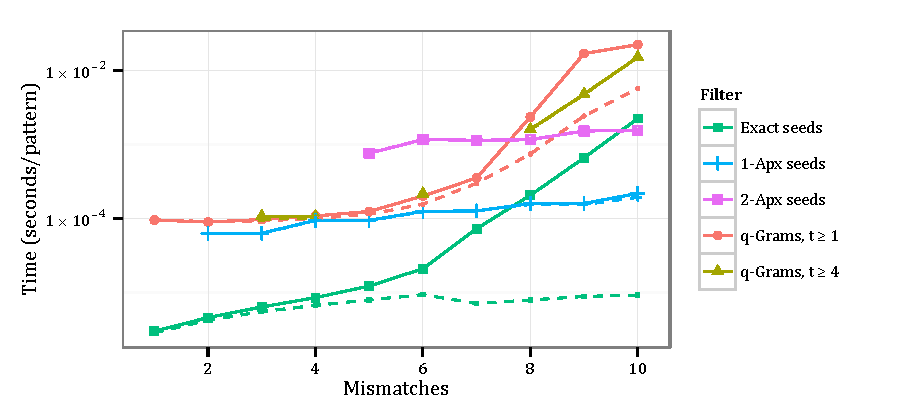
\includegraphics{filter_runtime.dna.celegans.hamming.100}
\end{center}
\end{figure}

\begin{figure}[t]
\begin{center}
\caption[Filters runtime on $k$-differences]{Filters runtime on $k$-differences. Pattern lengths are fixed to 100~bp. Solid lines represent total runtimes, while dashed lines represent filtration times only.}
\label{fig:filter-runtime-edit-celegans}
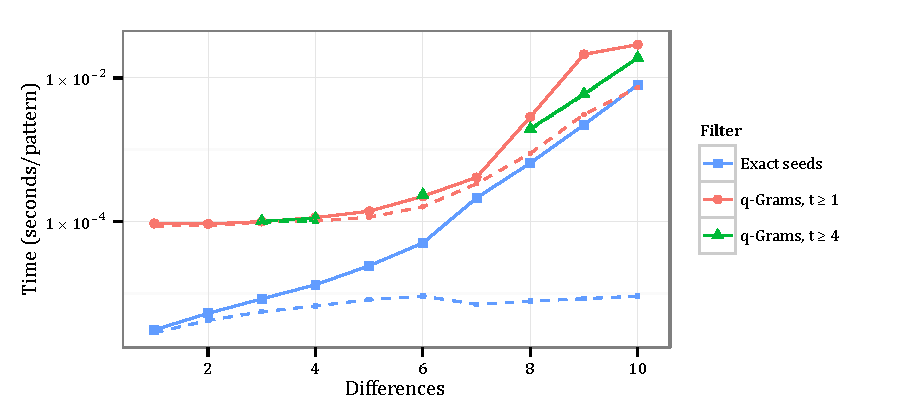
\includegraphics{filter_runtime.dna.celegans.edit.100}
\end{center}
\end{figure}

\subsection{Verification versus filtration time}

Figure \ref{fig:filter-ratio-hamming-celegans} shows the ratios between the runtimes of the verification and filtration phases of each filtration scheme.
For $k \leq 6$, all schemes spend more time on filtration rather than verification.
The weakest scheme, filtration with exact seeds, shows the closest ratio to 1.
As shown in the runtime plots (figures \ref{fig:filter-runtime-hamming-celegans}-\ref{fig:filter-runtime-edit-celegans}), quick filtration pays off for low error rates.
Here, a quicker full-text index would be beneficial.
For $k \geq 7$, contiguous $q$-grams with $\Threshold \geq 1$ show the closest ratio to 1, nonetheless the fastest alternative is provided by filtration with 1-approximate seeds, for which only 10\,\% of the runtime goes in verifications.
Here, a judicious mix of exact and 1-approximate seeds could improve the total runtime.
The ratios for $k$-difference show analogous patterns (data not shown).

\begin{figure}[b]
\begin{center}
\caption[Filtration versus verification time on $k$-mismatches]{Filtration versus verification time on $k$-mismatches. Pattern lengths are fixed to 100~bp.}
\label{fig:filter-ratio-hamming-celegans}
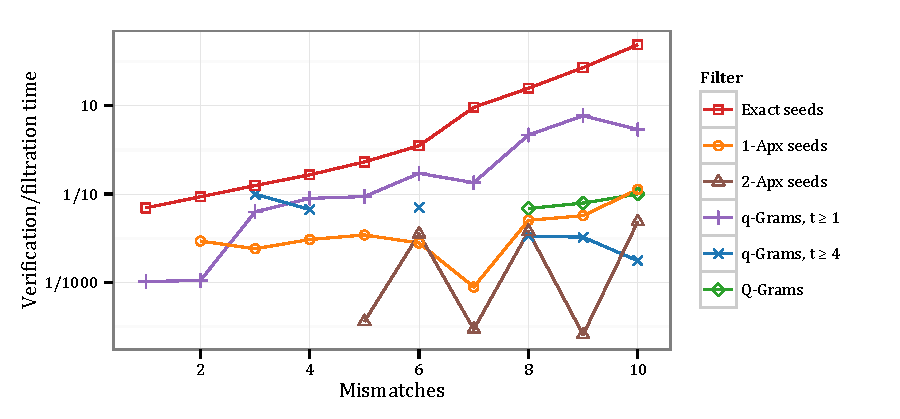
\includegraphics{filter_ratio.dna.celegans.hamming.100}
\end{center}
\end{figure}

%\begin{figure}[h]
%\begin{center}
%\caption[Ratio on $k$-differences]{Ratio on $k$-differences. Pattern length is fixed to 100.}
%\label{fig:filter-ratio-edit-celegans}
%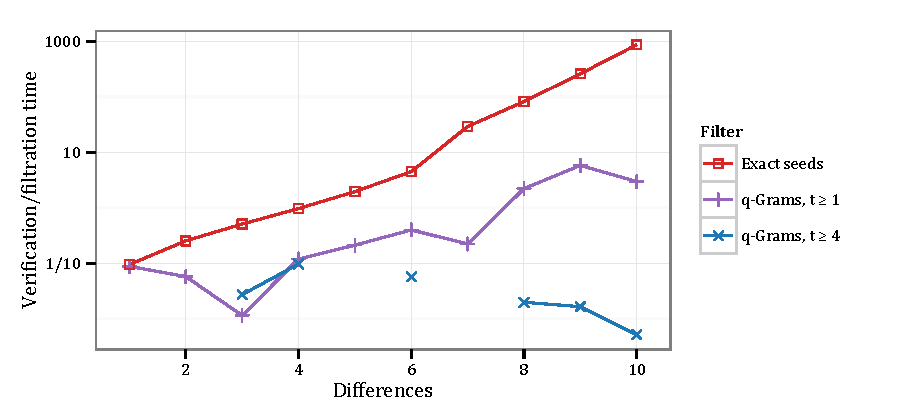
\includegraphics{filter_ratio.dna.celegans.edit.100}
%\end{center}
%\end{figure}

\subsection{Positive predictive value}

Instead of measuring filtration specificity, as introduced in section \ref{intro:filtering:spec-sens}, I measure the \emph{positive predictive value} (PPV).
As shown in table \ref{tab:filter:ppv}, I define \emph{true positives} (TP), \emph{false positives} (FP), \emph{true negatives} (TN), or \emph{false negatives} (FN) in terms of the number of verifications $V_f(\Text)$ produced in the filtration phase and the number of approximate occurrences $C(\Text)$ of the pattern in the text.
Therefore, I define the PPV as:
\begin{eqnarray}
\frac{|TP_f(\Text)|}{|TP_f(\Text)| + |FP_f(\Text)|} = \frac{C(\Text)}{V_f(\Text)}
\end{eqnarray}

\begin{table}[t]
\begin{center}
\caption[Measurement of filtering methods efficiency]{Measurement of filtering methods efficiency. $V_f(\Text)$ counts the number of verifications, $C(\Text)$ the number of approximate occurrences, and $|\Text|$ the text length. Since all considered filtering methods are full-sensitive, the number of false negatives is always 0.}
\begin{tabular}{rcc}
\toprule
  & Positive & Negative\\
\midrule
True & $C(\Text)$ & $|\Text| - C(\Text)$ \\
False & $V_f(\Text) - C(\Text)$ & 0		\\
\bottomrule
\end{tabular}
\label{tab:filter:ppv}
\end{center}
\end{table}

Figure \ref{fig:filter-ppv-hamming-celegans} shows the results for $k$-mismatches.
As expected, 2-approximate seeds have always the highest PPV, followed by 1-approximate seeds.
The PPV of gapped $q$-grams is comparable to that of 2-approximate seeds, while that of contiguous $q$-grams with $\Threshold \geq 1$ oscillates around that one of exact seeds.
In particular, when $\Threshold$ approaches $1$, \eg for $k = 9$, the PPV of contiguous $q$-grams stays below that one of exact seeds.
Enforcing $\Threshold \geq 4$ boosts the PPV of contiguous $q$-grams to that one of 1-approximate seeds.
The PPVs for $k$-difference show analogous patterns (data not shown).

\begin{figure}[b]
\begin{center}
\caption[Filters specificity on $k$-mismatches]{Filters specificity on $k$-mismatches. Pattern lengths are fixed to 100~bp.}
\label{fig:filter-ppv-hamming-celegans}
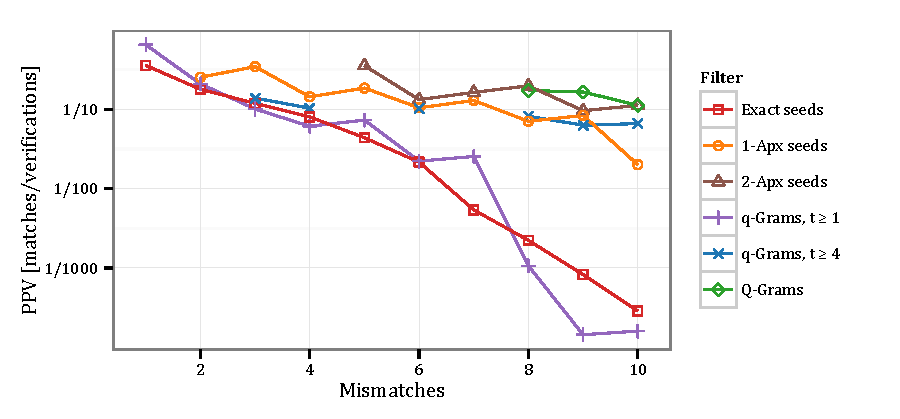
\includegraphics{filter_ppv.dna.celegans.hamming.100}
\end{center}
\end{figure}

%\begin{figure}[h]
%\begin{center}
%\caption[Filters specificity on $k$-differences]{Filters specificity on $k$-differences. Pattern length is fixed to 100.}
%\label{fig:filter-ppv-edit-celegans}
%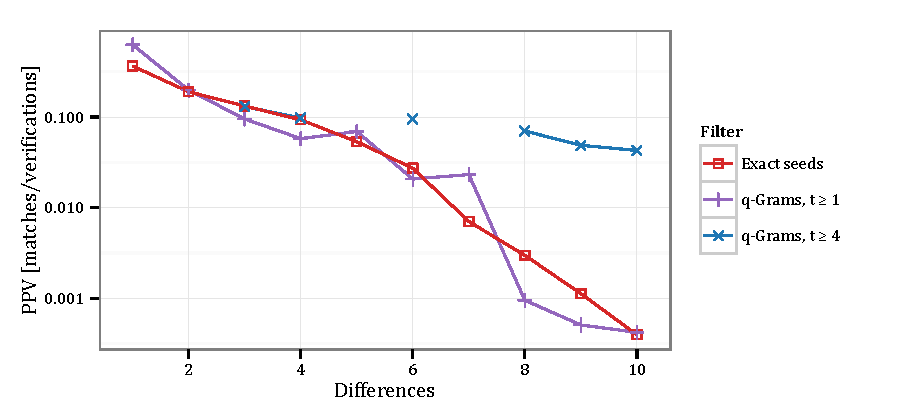
\includegraphics{filter_ppv.dna.celegans.edit.100}
%\end{center}
%\end{figure}
